\chapter{Summary and Conclusion}
\label{chapter: Conclusion}

The success or failure of a machine learning or deep learning process is directly proportional to the quality of the data used. The data source for this work, the \textit{2019 ISIC dataset}, presented several problems that required some treatment application to ensure the \textbf{elimination of biases} and to improve the project's viability. On one hand, the data was collected from different medical sources with different resolutions. On the other hand, there was a very significant difference in the number of elements per class, resulting in a very \textbf{unbalanced dataset}. In the first case, the images were transformed to the resolution required by the neural networks. In the second case, two different strategies were used: One consisted of trimming the samples according to the maximum number in the minority class (under-sampling technique). This approach is easy to apply, although its disadvantage causes the loss of richness by discarding data that could improve the model's metrics. To compensate this, we have opted for a second option: enriching the minority classes with synthetic images using SMOTE (\textbf{over-sampling} technique). This procedure has allowed us to increase the total number of images processed from 250 per class to 300, an increase of 20\%. In both options, it has been possible to train the models with a balanced dataset. 

To train the models, we used the \textbf{transfer learning} techniques. For this purpose, a classifier has been assembled using a \textbf{feature extractor} based on two well-known networks on the market, \textit{EfficientNet B0} and \textit{ResNet50}. This architecture was loaded with the weights of the \textit{ImageNet} dataset. This has allowed us to take advantage of the extractor's pattern recognition capabilities, complemented with a classifier stage. During the evolution of this work, the three steps of the transfer learning process have been demonstrated, showing in the second step, a substantial improvement of the network classification metrics was achieved.

In addition to the previous, two assembled networks have been tested with the two treated datasets; the first has been pruned, and the second the number of samples has been increased artificially employing SMOTE. As a result, we have observed while the EfficientNet-based classifier does not show any significant difference between training with one or the other dataset, the ResNet50-based network improves its metrics when trained with the SMOTE-based dataset. One possible explanation for this can be found by comparing the \textbf{depth of these networks}. Indeed, if we examine the right-hand column of the table \ref{tbl: Metrics summary}, we can see a significant difference in the number of training parameters ResNet50 versus EfficienNet B0. Thus, a deeper network such as ResNet would benefit from training with a larger dataset.

\section{Metrics summary}

% Please add the following required packages to your document preamble:
% \usepackage{graphicx}
% \usepackage[table,xcdraw]{xcolor}
% Beamer presentation requires \usepackage{colortbl} instead of \usepackage[table,xcdraw]{xcolor}
\begin{table}[ht]
\centering
\resizebox{\textwidth}{!}{%
\begin{tabular}{l|cc|cc|cc|cc|cc|ccc}
\cline{2-11}
 & \multicolumn{2}{c|}{\cellcolor[HTML]{EFEFEF}\textbf{Acc}} & \multicolumn{2}{c|}{\cellcolor[HTML]{EFEFEF}\textbf{Sen}} & \multicolumn{2}{c|}{\cellcolor[HTML]{EFEFEF}\textbf{Esp}} & \multicolumn{2}{c|}{\cellcolor[HTML]{EFEFEF}\textbf{F1-score}} & \multicolumn{2}{c|}{\cellcolor[HTML]{EFEFEF}\textbf{Time (sec)}} & \multicolumn{1}{l}{} & \multicolumn{1}{l}{} & \multicolumn{1}{l}{} \\ \hline
\rowcolor[HTML]{EFEFEF} 
\multicolumn{1}{|l|}{\cellcolor[HTML]{EFEFEF}\textbf{Model name}} & \multicolumn{1}{c|}{\cellcolor[HTML]{EFEFEF}\textbf{\begin{tabular}[c]{@{}c@{}}No \\ SMOTE\end{tabular}}} & \textbf{\begin{tabular}[c]{@{}c@{}}With \\ SMOTE\end{tabular}} & \multicolumn{1}{c|}{\cellcolor[HTML]{EFEFEF}\textbf{\begin{tabular}[c]{@{}c@{}}No\\ SMOTE\end{tabular}}} & \textbf{\begin{tabular}[c]{@{}c@{}}With\\ SMOTE\end{tabular}} & \multicolumn{1}{c|}{\cellcolor[HTML]{EFEFEF}\textbf{\begin{tabular}[c]{@{}c@{}}No\\ SMOTE\end{tabular}}} & \textbf{\begin{tabular}[c]{@{}c@{}}With\\ SMOTE\end{tabular}} & \multicolumn{1}{c|}{\cellcolor[HTML]{EFEFEF}\textbf{\begin{tabular}[c]{@{}c@{}}No\\ SMOTE\end{tabular}}} & \textbf{\begin{tabular}[c]{@{}c@{}}With\\ SMOTE\end{tabular}} & \multicolumn{1}{c|}{\cellcolor[HTML]{EFEFEF}\textbf{\begin{tabular}[c]{@{}c@{}}No\\ SMOTE\end{tabular}}} & \textbf{\begin{tabular}[c]{@{}c@{}}With\\ SMOTE\end{tabular}} & \multicolumn{1}{c|}{\cellcolor[HTML]{EFEFEF}\textbf{\# Epochs}} & \multicolumn{1}{c|}{\cellcolor[HTML]{EFEFEF}\textbf{\begin{tabular}[c]{@{}c@{}}\# Trainable \\ params\end{tabular}}} & \multicolumn{1}{c|}{\cellcolor[HTML]{EFEFEF}\textbf{\begin{tabular}[c]{@{}c@{}}\# Total \\ params\end{tabular}}} \\ \hline
\multicolumn{1}{|l|}{\cellcolor[HTML]{EFEFEF}\textbf{model ENetB0 1}} & \multicolumn{1}{c|}{0.39} & 0.40 & \multicolumn{1}{c|}{0.40} & 0.45 & \multicolumn{1}{c|}{0.39} & 0.40 & \multicolumn{1}{c|}{0.38} & 0.39 & \multicolumn{1}{c|}{3191} & 3560 & \multicolumn{1}{c|}{40} & \multicolumn{1}{c|}{12808} & \multicolumn{1}{c|}{4064939} \\ \hline
\multicolumn{1}{|l|}{\cellcolor[HTML]{EFEFEF}\textbf{model ENetB0 2}} & \multicolumn{1}{c|}{0.45} & 0.40 & \multicolumn{1}{c|}{0.43} & 0.45 & \multicolumn{1}{c|}{0.44} & 0.40 & \multicolumn{1}{c|}{0.41} & 0.39 & \multicolumn{1}{c|}{2017} & 625 & \multicolumn{1}{c|}{8} & \multicolumn{1}{c|}{1361208} & \multicolumn{1}{c|}{4064939} \\ \hline
\multicolumn{1}{|l|}{\cellcolor[HTML]{EFEFEF}\textbf{model ENetB0 3}} & \multicolumn{1}{c|}{0.57} & 0.51 & \multicolumn{1}{c|}{0.59} & 0.54 & \multicolumn{1}{c|}{0.57} & 0.50 & \multicolumn{1}{c|}{0.55} & 0.49 & \multicolumn{1}{c|}{2925} & 3244 & \multicolumn{1}{c|}{40} & \multicolumn{1}{c|}{4020356} & \multicolumn{1}{c|}{4064939} \\ \hline
\multicolumn{1}{|l|}{\cellcolor[HTML]{EFEFEF}\textbf{model RNet1}} & \multicolumn{1}{c|}{0.27} & 0.31 & \multicolumn{1}{c|}{0.27} & 0.31 & \multicolumn{1}{c|}{0.27} & 0.31 & \multicolumn{1}{c|}{0.27} & 0.30 & \multicolumn{1}{c|}{2851} & 2266 & \multicolumn{1}{c|}{30} & \multicolumn{1}{c|}{20488} & \multicolumn{1}{c|}{23589384} \\ \hline
\multicolumn{1}{|l|}{\cellcolor[HTML]{EFEFEF}\textbf{model RNet2}} & \multicolumn{1}{c|}{0.80} & 0.83 & \multicolumn{1}{c|}{0.81} & 0.84 & \multicolumn{1}{c|}{0.80} & 0.82 & \multicolumn{1}{c|}{0.80} & 0.82 & \multicolumn{1}{c|}{179} & 210 & \multicolumn{1}{c|}{5} & \multicolumn{1}{c|}{15250440} & \multicolumn{1}{c|}{23589384} \\ \hline
\multicolumn{1}{|l|}{\cellcolor[HTML]{EFEFEF}\textbf{model RNet3}} & \multicolumn{1}{c|}{0.94} & 0.98 & \multicolumn{1}{c|}{0.94} & 0.98 & \multicolumn{1}{c|}{0.94} & 0.98 & \multicolumn{1}{c|}{0.94} & 0.97 & \multicolumn{1}{c|}{354} & 497 & \multicolumn{1}{c|}{8} & \multicolumn{1}{c|}{23539848} & \multicolumn{1}{c|}{23589384} \\ \hline
\end{tabular}%
}
    \caption{Table summarising  each model metrics}
    \label{tbl: Metrics summary}
\end{table}

This table \ref{tbl: Metrics summary} shows the global metrics values of different training sessions. The first column on the left shows the name followed by a suffix indicating the step within the transfer learning process pointed out in the section \ref{ch:Transfer_learning}. We included two columns for each metric reflecting the obtained value when the model was trained with the balanced dataset after under-sampling (identified as "No SMOTE"). The second one is when the training was performed with the extended dataset by over-sampling (identified as "With SMOTE"). In addition to the classical classification metrics, another column was inserted with the training duration and the epochs number. We observed that calculating the quotient between both values could allow us to extract the time per epoch, which can help making a prediction of the training duration in case it would be necessary to extend the number of epochs required. 

Also, in this table, as we examined the accuracy and \textbf{F1-score} the first model values, it can be empirically proven that it did not improve when it was trained with the SMOTE-enriched dataset. The opposite can be seen when observing the values evolution on the second network, with a significant increase between the first and second steps, achieving good results in the third step. A comparison among the obtained results with both networks can be seen in the last step, the third. We saw a significant difference among them, which we obtained using EfficientNet B0, in the best case, with 57 \% accuracy, compared to 98 \% obtained by the ResNet50 network. Furthermore, in the third step, this model obtained \textbf{well-balanced metrics}, both in sensitivity and specificity, translating them into a high F1-score value; because of that, we considered it an excellent multiclass classifier.

\section{Sample prediction}

\begin{figure}[ht]
    \centering
        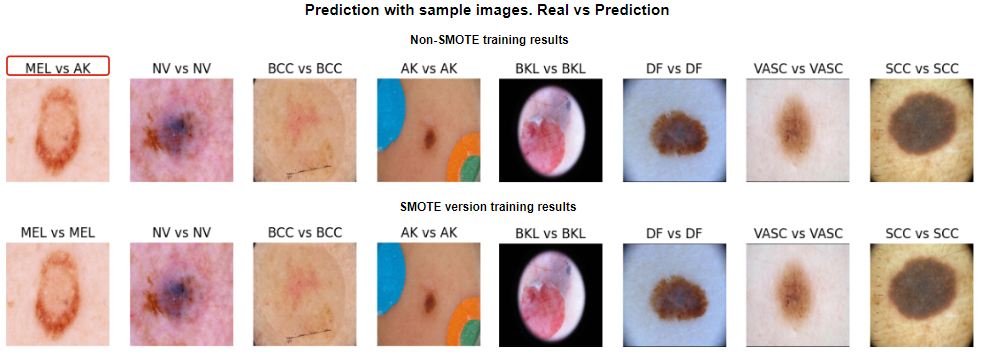
\includegraphics[scale=0.60]{images/Conclusion/Sample images Real vs Prediction.png}
        \caption{Test with a selection of sample images. Actual vs. Prediction Comparison}
    \label{fig: Sample Images real vs prediction}
\end{figure}

Finally, we have tested the ResNet50-based model predictive capacity, which provided the best results in our study. In order to test it, one image from each class of the test dataset was randomly selected from the test dataset. To follow the same line as the one used throughout our work, two models were used: the model trained with the dataset that has been sub-sampled and the one that was over-sampled with SMOTE. The results can be seen in the figure \ref{fig: Sample Images real vs prediction}. In the first image line, we have the predictions obtained after using the model trained with the first dataset, obtaining a success rate of seven out of the eight samples. In fact, to be easily distinguished, we marked the wrong value in a red box. The second row shows the predictions obtained using the same trained model with the dataset treated with SMOTE, where the Convolutional network obtained a success of 100 \%

\section{Suggestions}

We would like to propose several lines of action to continue the work done:
\begin{itemize}
    \item The first and most urgent action is to increase the number of synthetic samples performed with SMOTE. The hypothesis to prove or refute would be to see the maximum value of synthetic samples possible before the network stops learning due to the sample degradation for the feature repetition, so as to find the ceiling of this over-sampling technique.
    \item The second item proposed is to perform tests using deeper networks different from ResNet 50. For example, a variant of the ResNet with 101 layers \cite{noauthor_resnet101_nodate} doubles the number of the parameters at about 44 million. It is also possible to test the VGG16 behavior \cite{simonyan_very_2015}, because it has approximately 138 million parameters, and we can even venture to test with a vision transformer (ViT) \cite{noauthor_papers_nodate}, which is an architecture different from the one used in this work, which attention mechanisms replace the convolutional layers. 
    \item Although we have seen that the second network capacity for classifying is high, another option could be working on filtering incorporation to eliminate or attenuate those undesired image elements, such as hairs or marks, to delimit the lesion.  
\end{itemize}



